\documentclass[10pt,usenames,dvipsnames]{beamer}
\usepackage[english]{babel}
\usepackage{euler}

\usetheme{boxes}
%\useoutertheme{essential}
\usecolortheme{seagull}
\usefonttheme{professionalfonts}
\usefonttheme{structurebold}
\setbeamertemplate{navigation symbols}{}
\setbeamertemplate{frametitle}
{
	\begin{centering}
		\vspace{1.5em}
		\LARGE
    \insertframetitle
    \par
    %\vspace{0.5em}
  \end{centering}
}
\setbeamerfont{title}{size=\huge}
\setbeamerfont{subtitle}{size=\Large}
\renewcommand{\thefootnote}{\textsf{\fnsymbol{footnote}}}

% footnote refs per frame
\AtBeginEnvironment{frame}{\setcounter{footnote}{0}}

\usepackage[no-math]{fontspec}

\usepackage{tikz}
\usepackage{listings}
\usepackage{relsize}
\usepackage{array}
\usepackage{booktabs}
\usepackage{ragged2e}
\usepackage{varwidth}
\usepackage{multicol}
\usepackage{amsmath}

\makeatletter
\newlength{\negph@width}%
\newcommand{\negphantom}[1]{%
\settowidth{\negph@width}{#1}%
\hspace{-\negph@width}%
}
\makeatother

\newcommand{\aligntext}[2]{%
#2\negphantom{#2}\hphantom{#1}%
}

\setmainfont{texgyretermes}[
  Path=../fonts/,
  Extension=.otf,
  UprightFont=*-regular,
  BoldFont=*-bold,
  ItalicFont=*-italic,
  BoldItalicFont=*-bolditalic]
\setsansfont{texgyreheros}[
  Path=../fonts/,
  Extension=.otf,
  UprightFont=*-regular,
  BoldFont=*-bold,
  ItalicFont=*-italic,
  BoldItalicFont=*-bolditalic]
\setmonofont{RecMono-Casual}[
  Path=../fonts/,
  Extension=.ttf,
  BoldFont=*Bold,
  ItalicFont=*Italic,
  BoldItalicFont=*BoldItalic]

\usetikzlibrary{arrows}
\usetikzlibrary{backgrounds}
\usetikzlibrary{chains}
\usetikzlibrary{fit}
\usetikzlibrary{positioning}
\usetikzlibrary{scopes}
\usetikzlibrary{trees}
\usetikzlibrary{automata}
\usetikzlibrary{positioning}
\usetikzlibrary{shapes.multipart}

\lstset{basicstyle=\ttfamily}
\newcommand{\txtinput}[2][\ttfamily]{\lstinputlisting[language=none,basicstyle=#1]{#2}}
\newcommand{\txtinline}[2][\ttfamily]{\lstinline[language=none,basicstyle=#1]!#2!}
\newcommand{\cinput}[2][\ttfamily]{\lstinputlisting[language=C,basicstyle=#1]{#2}}
\newcommand{\cinline}[2][\ttfamily]{\lstinline[language=C,basicstyle=#1]!#2!}
\newcommand{\cppinput}[2][\ttfamily]{\lstinputlisting[language=C++,basicstyle=#1]{#2}}
\newcommand{\cppinline}[2][\ttfamily]{\lstinline[language=C++,basicstyle=#1]!#2!}
\newcommand{\llvminput}[2][\ttfamily]{\lstinputlisting[language=LLVM,basicstyle=#1]{#2}}
\newcommand{\llvminline}[2][\ttfamily]{\lstinline[language=LLVM,basicstyle=#1]!#2!}
\newcommand{\asminput}[2][\ttfamily]{\lstinputlisting[language=x86gas,basicstyle=#1]{#2}}
\newcommand{\asminline}[2][\ttfamily]{\lstinline[language=x86gas,basicstyle=#1]!#2!}
\lstdefinelanguage{LLVM}%
  {morekeywords={define,declare,global,constant,internal,external,private,%
      linkonce,linkonce_odr,weak,weak_odr,appending,common,extern_weak,%
      thread_local,dllimport,dllexport,hidden,protected,default,except,deplibs,%
      volatile,fastcc,coldcc,cc,ccc,x86_stdcallcc,x86_fastcallcc,ptx_kernel,%
      ptx_device,signext,zeroext,inreg,sret,nounwind,noreturn,nocapture,byval,%
      nest,readnone,readonly,noalias,uwtable,inlinehint,noinline,alwaysinline,%
      optsize,ssp,sspreq,noredzone,noimplicitfloat,naked,alignstack,module,asm,%
      align,tail,to,addrspace,section,alias,sideeffect,c,gc,target,datalayout,%
      triple,blockaddress},%
  morekeywords=[2]{add,fadd,sub,fsub,mul,fmul,sdiv,udiv,fdiv,srem,urem,frem,%
     and,or,xor,icmp,fcmp,eq,ne,ugt,uge,ult,ule,sgt,sge,slt,sle,oeq,ogt,oge,%
     olt,ole,one,ord,ueq,ugt,uge,ult,ule,une,uno,nuw,nsw,exact,inbounds,phi,%
     call,select,shl,lshr,ashr,va_arg,trunc,zext,sext,fptrunc,fpext,fptoui,%
     fptosi,uitofp,sitofp,ptrtoint,inttoptr,bitcast,ret,br,indirectbr,switch,%
     invoke,unwind,unreachable,malloc,alloca,free,load,store,getelementptr,%
     extractelement,insertelement,shufflevector,extractvalue,insertvalue},%
  sensitive=t,%
  morestring=[b]",%
  morecomment=[l];%
  }[keywords,comments,strings]
\lstdefinelanguage{x86gas}%
  {morekeywords={%
.abort, .ABORT, .align, .ascii, .asciz, .balign, .bss, .bundle, .byte, .cfi, %
.comm, .cstring, .data, .def, .desc, .dim, .double, .eject, .else, .elseif, %
.end, .endef, .endfunc, .endif, .equ, .equiv, .eqv, .err, .error, .exitm, %
.extern, .fail, .file, .fill, .float, .func, .global, .globl, .gnu, .hidden, %
.hword, .ident, .if, .incbin, .include, .int, .internal, .irp, .irpc, .lcomm, %
.lflags, .line, .ln, .linkonce, .list, .loc, .local, .long, .macro, .mri, %
.noaltmacro, .nolist, .octa, .offset, .org, .p2align, .popsection, .previous, %
.print, .protected, .psize, .purgem, .pushsection, .quad, .rept, .sbttl, .scl, %
.section, .set, .short, .single, .size, .skip, .sleb128, .space, .stabd, %
.stabn, .stabs, .string, .struct, .subsection, .symver, .tag, .text, .title, %
.type, .uleb128, .val, .version, .vtable, 	.vtable_entry, 	.vtable_inherit, %
.warning, .weak, .weakref, .word, .zero
},%
  morekeywords=[2]{%
aaa, adcb, adcl, add, addb, addl, addps, addw, addq, adds, addss, addsd, and, %
andb, andw, andl, andq, bswap, call, callq, cld, cltd, cltq, cmova, cmovae, %
cmovb, cmovbe, cmovg, cmovge, cmovl, cmovle, cmovna, cmovnae, cmovnb, cmovnbe, %
cmovne, cmovng, cmovnge, cmovnl, cmovnle, cmovns, cmovnz, cmovs, cmovz, cmp, %
cmpb, cmpeqps, cmpl, cmpq, cmpsl, cmpxchg, cpuid, cqto, cvtps2dq, cvtdq2ps, %
cvtsd2ss, cvtsi2s, cvtsi2ss, cvtsi2ssq, cvtsi2sd, cvtsi2sdq, cvtss2sd, cvttsd, %
cvttsd2si, cvttsd2siq, cvtts, cvttss, cvttss2si, cvttss2siq, das, dec, decb, %
decw, decl, decq, divw, divl, divq, divs, divss, divsd, fabs, fadd, fbld, %
fbstp, fchs, fcmovb, fcomi, fcoms, fcos, fdivp, fdivr, fdivrp, fidivs, filds, %
fimul, finit, fists, fld1, fldcw, fldl, fldl2t, fldl2e, fldlenv, fldlcw, %
fldlg2, fldln2, fldpi, flds, fldz, fmul, fmulp, fprem1, frame, frndint, %
frstor, fsave, fsin, fsincos, fsqrt, fst, fstcw, fstl, fstps, fsts, fstsw, %
fstenv, fstpl, fstsw, fsubr, fxch, fyl2x, idivl, idivq, imul, imulb, imull, %
imulw, imulq, inc, incb, incw, incl, incq, int, ja, jb, jc, jcxz, je, jg, jge, %
jl, jmp, jne, jns, jnz, jo, jp, js, jz, lea, leab, leave, leawl, leaq, leal, %
lodsb, lodsl, loop, maxps, maxs, maxss, maxsd, mins, minss, minssd, mov, %
movabsq, movapd, movaps, movqps, movb, movdqa, movdqu, movl, movlpd, movq, %
movupd, movups, movsb, movsbw, movsbl, movsbq, movsd, movsl, movslq, movsw, %
movswl, movswq, movsx, movss, movsd, movw, movz, movzbw, movzbl, movzbq, %
movzwl, movzwq, movzx, msg, mull, mulpd, muls, mulss, mulsd, mulq, neg, negb, %
negw, negl, negq, nop, not, notb, notw, notl, notq, or, orb, orw, orl, orq, %
paddd, pcmpeqw, pop, popfl, popl, popq, popw, push, pushfl, pushl, pushq, %
pushw, rep, repe, repne, ret, retq, rspreg, sahf, sal, salb, salw, sall, salq, %
sar, sarb, sarw, sarl, sarq, sbbb, sbbl, shr, shrb, shrw, shrl, shrq, sqrtps, %
sqrts, sqrtss, sqrtsd, std, stosb, sub, subb, subl, subq, subw, subs, subss, %
subsd, syscall, test, testb, testq, ucomis, ucomisd, ucomiss, xchg, xor, xorb, %
xorps, xorw, xorl, xorq, vxorpd, vaddsd},%
  sensitive=t,%
  morestring=[b]",%
  morecomment=[l]\#%
  }[keywords,comments,strings]
\lstdefinelanguage{none}{
  identifierstyle=
}
  
% Create Color definition From Template: 
% #1 template name, 
% #2 foreground color name
% #3 background color name
\newcommand{\ccft}[3]{
\usebeamercolor{#1}
\definecolor{#2}{named}{fg}
\definecolor{#3}{named}{bg}
}
\ccft{palette primary}{ThemePriFg}{ThemePriBg}
\ccft{palette secondary}{ThemeSecFg}{ThemeSecBg}
\ccft{palette tertiary}{ThemeTerFg}{ThemeTerBg}
\ccft{palette quaternary}{ThemeQuaFg}{ThemeQuaBg}



\author{Daniele Cattaneo}
\institute{Politecnico di Milano}
\date{\DATE}
\title{The LLVM compiler framework}
\subtitle{Introduction}
\newcommand{\customdata}{Daniele Cattaneo <daniele.cattaneo@polimi.it>}

\AtBeginSection[]
{
\begin{frame}{Contents}
\tableofcontents[currentsection,subsectionstyle=show/shaded/hide]
\end{frame}
}

\AtBeginSubsection[]
{
\begin{frame}{Contents}
\tableofcontents[currentsection,subsectionstyle=show/shaded/hide]
\end{frame}
}

\begin{document}


\begin{frame}
\maketitle
\begin{center}
\itshape\scriptsize
These slides were originally written by
Michele Scandale, Ettore Speziale and Stefano Cherubin for the
``Code Transformation and Optimization'' course.
\end{center}
\end{frame}


% !TEX root = main.tex

\section{Introduction}


\begin{frame}{Understanding LLVM}
	\begin{center}
	\huge{
		LLVM is \textbf{not} a compiler.\\
		\pause
		\vfill
		LLVM is a\\\textbf{collection of components}\\
		which is \textbf{useful}\\to build a compiler.
	}
	\end{center}
\end{frame}


\begin{frame}{Getting LLVM}
\begin{itemize}
	\item ``old'' git mirrors
		\begin{itemize}
			\item only llvm repo (subprojects in separated repos, can be added later)
			\item \texttt{git clone -b release\_90 --single-branch git@github.com:llvm-mirror/llvm.git}
		\end{itemize}
	\vfill
	\item ``new'' git monorepo
		\begin{itemize}
			\item all in one repo (llvm + major subprojects)
			\item \texttt{git clone -b release/9.x --single-branch git@github.com:llvm/llvm-project.git}
		\end{itemize}
\end{itemize}
\end{frame}


\begin{frame}{What LLVM is made of}
\begin{itemize}
	\item C++ libraries
		\begin{itemize}
			\item \texttt{src/include/llvm/...}
			\item \texttt{src/lib/...}
		\end{itemize}
		\vfill
	\item small application (tools)
		\begin{itemize}
			\item \texttt{src/tools/...}
			\item \texttt{src/utils/...}
		\end{itemize}
\end{itemize}
\vfill
You can find binaries of them in the installation directory under \texttt{root/bin/...}
\end{frame}


\begin{frame}{clang}
\begin{itemize}
	\item \texttt{clang} is a compiler based on LLVM
	\item It compiles all major C-like languages
	\vfill
	\item It is part of the git monorepo
	\item It can be added as a tool in the LLVM framework but must be manually cloned in the tool directory
	\begin{enumerate}
		\item \texttt{cd src/tools}
		\item \texttt{git clone http://llvm.org/git/clang} (git mirror version)
	\end{enumerate}
	\vfill
	\item You can easily see on a production quality compiler the impact of changes you made on your local copy of LLVM
\end{itemize}
\end{frame}


\begin{frame}{Commands}
	\begin{description}[llvm-dwarfdump]
		\item[llvm-as] LLVM assembler
		\item[llvm-dis] LLVM disassembler
		\item[opt] LLVM optimizer
		\item[llc] LLVM static compiler
		\item[lli] directly execute programs from LLVM bitcode
		\item[llvm-link] LLVM bitcode linker
		\item[llvm-mca] LLVM machine code analyzer
		\item[llvm-nm] list LLVM bitcode and object file's symbol table
		\item[llvm-stress] generate random .ll files
		\item[llvm-config] prints out install configuration parameters
		\item[llvm-dwarfdump] print contents of DWARF sections
	\end{description}
	\vfill
	For a complete reference, see the LLVM command guide\footnote{\url{http://llvm.org/docs/CommandGuide/index.html}}
\end{frame}



% !TEX root = main.tex

\section{Compiler organization}


\begin{frame}{Compiler pipeline}
\begin{center}
Typically a compiler is a \alert{pipeline}.\\
\bigskip
Advantages of the pipeline model:\\
\medskip
\begin{varwidth}{0.8\textwidth}
\begin{itemize}
\item \alert{simplicity} -- read something, produce something
\item \alert{locality} -- no superfluous state
\end{itemize}
\end{varwidth}
\\
\bigskip
Complexity lies on \alert{chaining} together stages.
\end{center}
\end{frame}


\begin{frame}{Compiler pipeline}{Internal pipelines}
\begin{center}
High-level pipeline structure of a compiler:\\
\begin{figure}
\centering

% compiler-structure.tex: generic organization of a compiler.

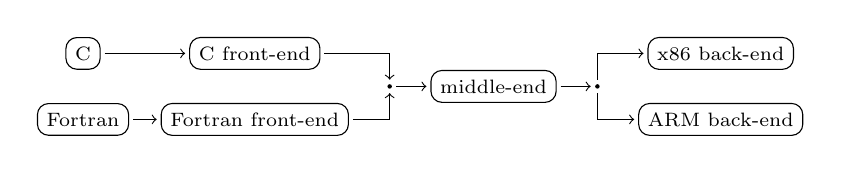
\begin{tikzpicture}
[
  every node/.style={
    font=\scriptsize
  },
  cell/.style={
    rectangle,
    rounded corners,
    draw
  },
  point/.style={
    circle,
    fill,
    inner sep=.2mm
  },
  tip/.style={
    ->,
    shorten >=.5mm,
    shorten <=.5mm
  },
  man-tip/.style={
    tip,
    to path={-| (\tikztotarget)}
  },
  rman-tip/.style={
    tip,
    to path={|- (\tikztotarget)}
  }
]

\matrix [column sep=4mm]
{
\node (c-language)   [cell] {C};             &
\node (c-front-end)  [cell] {C front-end};   &
\node ()             []     {};              &
\node ()             []     {};              &
\node ()             []     {};              &
\node (x86-back-end) [cell] {x86 back-end}; \\

\node ()               []      {};           &
\node ()               []      {};           &
\node (middle-end-in)  [point] {};           &
\node (middle-end)     [cell]  {middle-end}; &
\node (middle-end-out) [point] {};           &
\node ()               []      {};          \\

\node (fortran-language)  [cell] {Fortran};           &
\node (fortran-front-end) [cell] {Fortran front-end}; &
\node ()                  []     {};                  &
\node ()                  []     {};                  &
\node ()                  []     {};                  &
\node (arm-back-end)      [cell] {ARM back-end};     \\
};

{ [start chain]
\chainin (c-language)    [join];
\chainin (c-front-end)   [join=by tip];
\chainin (middle-end-in) [join=by man-tip];
}

{ [start chain]
\chainin (fortran-language)  [join];
\chainin (fortran-front-end) [join=by tip];
\chainin (middle-end-in)     [join=by man-tip];
}

{ [start chain]
\chainin (middle-end-in)  [join];
\chainin (middle-end)     [join=by tip];
\chainin (middle-end-out) [join=by tip];
}

{ [start chain]
\chainin (middle-end-out) [join];
\chainin (x86-back-end)   [join=by rman-tip];
}

{ [start chain]
\chainin (middle-end-out) [join];
\chainin (arm-back-end)   [join=by rman-tip];
}
\end{tikzpicture}

\end{figure}
\medskip
There are three main components:

\begin{description}
\item[Front-end] \alert{translates} a source file into the intermediate representation
\item[Middle-end] \alert{analyzes} the intermediate representation, \alert{optimizes}
                  it
\item[Back-end] \alert{generates} target machine assembly from the intermediate
                representation
\end{description}
\end{center}
\end{frame}


\begin{frame}{The LLVM compiler pipeline}
\begin{center}
We will consider only the \emph{middle-end}.\\
{\small Same concepts are valid also for \{front,back\}-end.}\\
\bigskip
\begin{description}[Pass Manager]
\item[IR] (a.k.a. Intermediate Representation) the \alert{language} used in the
          middle-end
\item[Pass] a \alert{pipeline stage}\\
a Pass may have \alert{dependencies} on other Passes.
\item[Pass Manager] component that \alert{schedules} passes according to their \alert{dependencies} and \alert{executes} them\\
\emph{(builds the pipeline)}
\end{description}
\end{center}
\end{frame}


\begin{frame}{First insights}
A compiler is \alert{complex}:

\begin{itemize}
\item passes are the \alert{elementary unit of work}
\item Pass Manager must be \alert{advised} about pass chaining
\item pipeline shapes are \alert{not fixed} -- they can change from one compiler
      execution to another\\
      {\small e.g. optimized/not optimized builds, compiler options, ...}
\end{itemize}
\end{frame}


\begin{frame}{A word of warning!}
\begin{center}
{\large 
Compilers must be \alert{conservative}:\\
\smallskip
$\Downarrow$\\
\smallskip
All passes \alert{must preserve the program semantics}\\
\smallskip
$\Downarrow$\\
\smallskip
Compiler passes must be designed \alert{very carefully}!\\
}
\end{center}
\end{frame}

% !TEX root = main.tex

\section{Algorithm design}


\begin{frame}{Classical Algorithm Design}
In algorithm design, a good approach is the following:
\begin{enumerate}
\item study the problem
\item make some example
\item identify the \alert{common case}
\item derive the algorithm for the common case
\item add handling for \alert{corner cases}
\item improve performance by \alert{optimizing the common case}
\end{enumerate}

\vfill
Weakness of the approach:
\begin{itemize}
\item \alert{corner cases}:\\a \emph{correct} algorithm \textbf{must} consider \emph{all the corner cases}!
\end{itemize}
\end{frame}


\begin{frame}{Compiler Algorithm Design}{Be Conservative}
\begin{center}
Corner cases are difficult to handle, but they cannot be ignored\\
\smallskip
{\small Compiler algorithms must be \alert{proven} to preserve\\
program semantic \alert{at all times}}\\
\bigskip
As an aid, a \emph{standard methodology} is employed.\\
\bigskip
Compiler algorithms are built combining \alert{three} kinds of passes:\\
\medskip
Analysis, Optimization, Normalization\\
\bigskip
\pause
We now consider a simple example: \emph{loop hoisting}.
\end{center}
\end{frame}


\begin{frame}{Loop Hoisting}
It is a transformation that:
\begin{itemize}
\item looks for statements (inside a loop) not depending on the loop state
\item move them outside the loop body
\end{itemize}

\begin{columns}[t]
\column{.45\textwidth}
\begin{block}{Loop Hoisting -- Before}
\centering
\cinput{snippet/loop-hoisting-before.c}
\end{block}

\column{.45\textwidth}
\begin{block}{Loop Hoisting -- After}
\centering
\cinput{snippet/loop-hoisting-after.c}
\end{block}
\end{columns}
\end{frame}


\begin{frame}{Loop Hoisting}{Focus on the Transformation}
\begin{block}{The general idea:}
\begin{itemize}
\item move ``good'' statement outside of the loop
\end{itemize}
\end{block}

This \alert{pass} modifies the code, thus it is an \alert{optimization pass}.

It needs to know:
\begin{itemize}
\item which pieces of code are loops
\item which statements are ``good'' statements
\end{itemize}

This information is computed by the the \alert{analysis} passes:

\begin{itemize}
\item detecting loops in the program
\item detecting loop-independent statements
\end{itemize}

The loop hoisting pass declares which analyses it needs:

\begin{itemize}
\item pipeline automatically built: \alert{analysis $\rightarrow$ optimization}
\end{itemize}
\end{frame}


\begin{frame}{Loop Hoisting}{Proving Program Semantic Preservation}
The \alert{proof} is trivial:

\begin{itemize}
\item the transformation shall preserve program semantics
\item the analyses shall be correct
\end{itemize}

Analysis passes are usually built starting from other analyses already
implemented inside the compiler, or are already present in LLVM
\begin{itemize}
\item often, no proof is necessary for the analyses
\end{itemize}

\vfill
\begin{center}
\alert{However...}\\
\smallskip
You also have to prove that the combination of analysis + transformation is correct!\\
\smallskip
"Beware of bugs in the above code;\\I have only proved it correct, not tried it."\\--- Knuth
\end{center}
\end{frame}


\begin{frame}{The importance of normalization}
\begin{center}
We have spoken about loops, but which kind of loop?\\
\medskip
\cinline{do-while}? \cinline{while}? \cinline{for}?\\

\bigskip
Almost all loops are different forms of the \alert{same exact thing}\\
$\Downarrow$\\
We can convert a lot of loops to a loop of another kind!\\

\bigskip
To account for the various kinds of loops, we choose a \alert{normal}
kind of loop, and then we write a \alert{normalization} pass.\\
\smallskip
{\footnotesize
Usually, \cinline{do-while} loops are chosen to be the \emph{normal} loops.\\
\vspace{-1mm}
Sometimes, normalization is also called \alert{canonicalization}.}\\

\bigskip
The more loops we recognize, the higher the potential\\
\alert{optimization impact}!
\end{center}
\end{frame}


\begin{frame}{A Methodology}
You have to:

\begin{enumerate}
\item analyze the problem
\item make some examples
\item detect the common case
\item determine the \alert{input conditions}
\item determine which \alert{analyses} you need
\item design the \alert{optimization} pass
\item proof its \alert{correctness}
\item improve algorithm perfomance on the common case
\item improve the effectiveness of the algorithm by adding
      \alert{normalization passes}
\end{enumerate}
\end{frame}


\begin{frame}{Ignore corner cases!}
\begin{center}
Something is missing...\\
\bigskip
{\Large Corner Cases!}\\
\bigskip
Why?\\
\end{center}
\begin{enumerate}
\item It makes no sense to optimize code that is seldom executed
\item Your optimization will be based on \alert{properties of the code that are true only in the common case you are considering}
\begin{itemize}
\item If the code does not fit the common case, it shall stay as-is
\item Otherwise you \alert{risk breaking program semantics}!
\end{itemize}
\end{enumerate}
\end{frame}


% !TEX root = main.tex

\section{Inside LLVM}


\begin{frame}{LLVM-IR is like a box of chocolates}{You never know what you're gonna get}
\begin{center}
LLVM-IR comes in 3 different flavours:
\end{center}
\bigskip
\begin{description}
\item[assembly] on-disk human-readable format\\(file extension: \texttt{.ll})
\item[bitcode] on-disk machine-oriented binary format\\(file extension: \texttt{.bc})
\item[in-memory] in-memory binary format\\(used during compilation process)
\end{description}
\bigskip
\begin{center}
All formats have the same expressiveness!
\end{center}
\vfill
\end{frame}


\begin{frame}{Using the driver to produce LLVM-IR}
\begin{center}
\vfill
We can generate LLVM-IR assembly using the \texttt{clang} driver:\\
\bigskip
\texttt{clang -emit-llvm -S -o out.ll in.c}\\
\medskip
{\footnotesize If you want to generate bitcode instead:\\
\texttt{clang -emit-llvm -o out.bc in.c}\\
}
\bigskip
The compiler driver can also generate native code starting from 
LLVM-IR assembly\\
\smallskip
{\small(Like compiling an assembly file with GCC)}
\vfill
\end{center}
\end{frame}


\begin{frame}{Playing with LLVM Passes}
Run one or more passes on the LLVM-IR on-demand by using \texttt{opt}:

\begin{itemize}
\item Syntax is like \texttt{clang} (supports even \texttt{-O1}, \texttt{-O2}...)
\item One command line argument per pass to run
\item Order of execution is the same as the argument order
\begin{itemize}
\item Different order, different results! (\alert{phase/stage ordering})
\end{itemize}
\end{itemize}

\vfill
Some useful passes for debugging (they do not transform anything):

{\small
\begin{description}[print dominator tree]
\item[print CFG] \texttt{opt -view-cfg input.ll}
\item[print dominator tree] \texttt{opt -view-dom input.ll}
\item[print current IR] \texttt{opt -print-module input.ll}
\end{description}
}

\vfill
\begin{example}
\begin{itemize}
\item Run \emph{mem2reg}, then view the CFG:
\begin{itemize}
\item \texttt{opt -mem2reg -view-cfg input.ll}
\end{itemize}
\end{itemize}
\end{example}
\end{frame}


\begin{frame}{Pass Hierarchy}
LLVM provides a lot of passes...

\begin{itemize}
\item Try \texttt{opt -help}!
\end{itemize}

\vfill
For performance reasons there are different kind of passes:

\begin{block}{LLVM Passes}

% llvm-passes: hierarchy of LLVM passes.

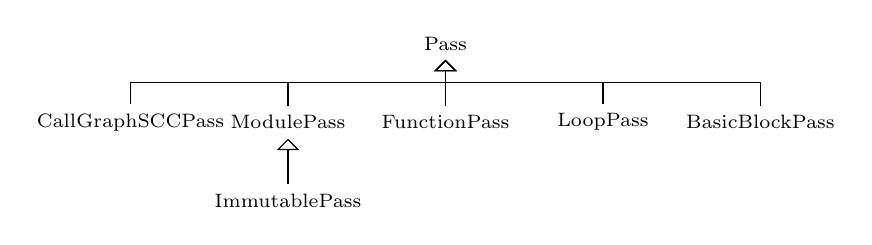
\begin{tikzpicture}
[
  every node/.style={
    font=\scriptsize
  },
  extends/.style={
    draw,
    open triangle 90-
  },
  level distance=10mm,
  level 1/.style={
    sibling distance=20mm
  },
  level 3/.style={
    sibling distance=20mm
  }
]

\node {Pass}
  [edge from parent fork down,
   edge from parent/.style={extends}]

  child { node {CallGraphSCCPass}}
  child { node {ModulePass}
    child { node {ImmutablePass}}
  }
  child { node {FunctionPass}}
  child {node {LoopPass}}
  child {node {BasicBlockPass}};
\end{tikzpicture}

\centering
\end{block}
\end{frame}


\begin{frame}{LLVM Passes}
Each kind of pass visits particular elements of a module:

\begin{description}[align=left, labelwidth=1cm]
\item[ImmutablePass] compiler configuration -- never run
\item[CallGraphSCCPass] post-order visit of CallGraph SCCs
\item[ModulePass] visit the whole module
\item[FunctionPass] visit functions
\item[LoopPass] post-order visit of loop nests
%\item[BasicBlockPass] visit basic blocks % DEPRECATED AND REMOVED
\item[RegionPass] visit a custom-defined region of code
\end{description}

\vfill
Specializations come with restrictions:

\begin{itemize}
\item e.g. a \alert{FunctionPass} cannot add or delete functions
\item refer to ``Writing a LLVM Pass''~\cite{LOCAL:www/llvmWritingAPass}
      for documentation on features and limitations of each kind of pass
\end{itemize}
\end{frame}


% \begin{frame}{Examples}
% Now we will see very simple passes:
%
% \begin{itemize}
% \item some of them are meaningless
% \item goal is to show you the LLVM API
% \end{itemize}
%
% \vfill
%
% The passes are:
% \begin{description}
% \item[instruction-count] simple instruction counting analysis
% \item[hello-llvm] optimization pass building an hello-world program
% \item[function-eraser] optimization pass removing ``small'' functions
% \end{description}
%
% \vfill
% Hint: take the LLVM pass writing tutorial~\cite{LOCAL:www/llvmWritingAPass}
% \end{frame}


\begin{frame}{Recap}
\begin{itemize}
\item The \alert{user} invokes the \alert{compiler} via the \alert{driver}
\item The \alert{compiler} is made of three \alert{stages}\\(front-end, middle-end, back-end)
\item The \alert{middle-end} is made of \alert{passes}
\end{itemize}
\medskip
If you want things done, you want to work on a \alert{pass}.\\
\medskip
\begin{itemize}
\item Edit an existing pass
\item Create a new pass
\end{itemize}
\medskip
To design a pass, you must follow the principle of \alert{conservativeness}.\\
\bigskip\centering\large
Next step: how to actually code a pass!
\end{frame}


% !TEX root = main.tex

\subsection{The LLVM-IR language}


\begin{frame}{How passes work}
\centering
A \alert{pass} is a \alert{subroutine} that \\programmatically
transforms a piece of code.\\
\bigskip
The code of the pass operates on the LLVM-IR \\using a set of
\alert{object-oriented APIs}.
\vfill
Let's examine the LLVM-IR~\cite{LOCAL:www/llvmLanguageRef} more closely,\\
first by looking at its \alert{human-readable} form.
\end{frame}


\begin{frame}{LLVM-IR}{Example: factorial}
\begin{center}
\begin{varwidth}{20cm}
\llvminput[\ttfamily\fontsize{7pt}{5pt}\selectfont]{snippet/fact.ll}
\end{varwidth}
\end{center}
\end{frame}


\begin{frame}{LLVM-IR}{What it looks like}
LLVM-IR looks a lot like a RISC assembly language:\\

\begin{itemize}
\item Few instructions, all perfectly orthogonal
	\begin{itemize}
	\item There are infinite registers
	\item There are no special-purpose registers
	\item No implicit flags register
	\end{itemize}
\item Basic block boundaries are denoted by \alert{labels}
\item Only \llvminline{load} and \llvminline{store} access memory
\end{itemize}

\vfill
There are also a few CISC-like \alert{high level instructions}:

\begin{itemize}
\item Reserve memory on the stack -- \llvminline{alloca}
\item Function call -- \llvminline{call}
	\begin{itemize}
	\item The calling convention is abstracted away
	\item There is an implicit call stack
	\end{itemize}
\item Pointer arithmetics -- \llvminline{getelementptr}
\item \ldots
\end{itemize}
\end{frame}


\begin{frame}{LLVM-IR}{How it is actually structured}
In reality LLVM-IR is much more high-level than assembly.
\begin{itemize}
\item The topmost object of a LLVM-IR program is the \alert{Module}.
\item \alert{Modules} contain a list of \alert{Globals}.
	\begin{itemize}
	\item {Globals} can be either \alert{Functions} or \alert{Global Variables}.
	\item A global can be a \alert{Forward declaration}.
	\end{itemize}
\item \alert{Functions} contain a list of \alert{Basic Blocks} + \alert{Arguments}.
\item \alert{Basic Blocks} are a list of \alert{Instructions}.
\end{itemize}
\begin{block}{The in-memory representation}
All these parts will correspond directly to \alert{C++ objects}.\\
The abundance of lists guarantees low overhead and scalability to very large programs.
\end{block}
\end{frame}


\begin{frame}{LLVM-IR}{Values \& Types}
LLVM-IR is \alert{strongly typed}:

\begin{itemize}
\item e.g. you cannot assign a floating point value to an integer register
without an explicit cast
\end{itemize}
\medskip
\alert{Almost everything} is \alert{typed}:\\
\medskip
\begin{tabular}{>{\RaggedLeft\arraybackslash}p{5.55em}lcl}
\textbf{functions} & \llvminline{@fact} & $\rightarrow$ & \llvminline{i32 (i32)} \\
\textbf{registers} & \llvminline{\%3 = icmp eq i32 \%2, 0} & $\rightarrow$ & \llvminline{i1} \\
\textbf{global vars.} & \llvminline{@var = common global i32 0} & $\rightarrow$ & \llvminline{i32} \\
\end{tabular}\\
\medskip
These objects that have a type are called (somewhat confusingly)\\\alert{LLVM Values}.
\begin{block}{The in-memory representation}
\cppinline{llvm::Value} is the \alert{base class} of almost all interesting LLVM-IR objects!
\end{block}
\end{frame}


\begin{frame}{LLVM-IR}{Hierarchy}
\centering
% !TEX root = ../main.tex
% class-hier: core class hierarchy of LLVM

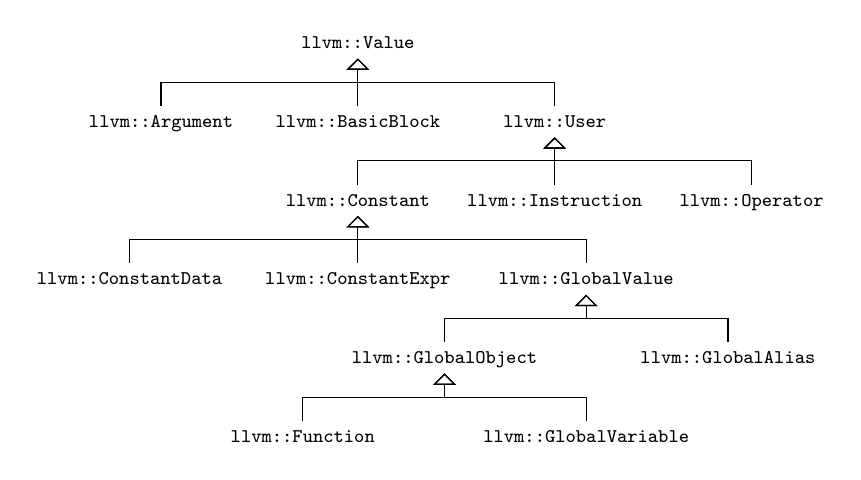
\begin{tikzpicture}
[
  every node/.style={
    font=\tt\scriptsize,
    text depth=0pt
  },
  extends/.style={
    draw,
    open triangle 90-
  },
  level distance=10mm,
  sibling distance=25mm,
  level 3/.style={
    sibling distance=29mm
  },
  level 4/.style={
    sibling distance=36mm
  },
]

\node{llvm::Value}
  [edge from parent fork down,
   edge from parent/.style={extends}]

  child{ node{\cppinline{llvm::Argument}} }
  child{ node{\cppinline{llvm::BasicBlock}} }
  child{ node{\cppinline{llvm::User}}
  	child{ node{\cppinline{llvm::Constant}}
			child{ node{\cppinline{llvm::ConstantData}} }
			child{ node{\cppinline{llvm::ConstantExpr}} }
			child{ node{\cppinline{llvm::GlobalValue}} 
				child{ node{\cppinline{llvm::GlobalObject}} 
					child{ node{\cppinline{llvm::Function}} }
					child{ node{\cppinline{llvm::GlobalVariable}} }
				}
				child{ node{\cppinline{llvm::GlobalAlias}} }
			}
		}
		child{ node{\cppinline{llvm::Instruction}} }
		child{ node{\cppinline{llvm::Operator}} }
  };
\end{tikzpicture}
\\
%\pause
%\bigskip
%Something is missing...
\end{frame}


\begin{frame}{LLVM-IR}{Static Single Assignment}
LLVM-IR is SSA-based:

\begin{itemize}
\item every register is \alert{statically assigned} exactly \alert{once}
\end{itemize}
\bigskip
Statically means that:

\begin{itemize}
\item inside each function...
\item ...for each register \llvminline{\%foo}...
\item ...there is \alert{only one} statement in the form \llvminline{\%foo = ...}
\end{itemize}
\bigskip
\alert{Static} (compile time) $\neq$ \alert{dynamic} (runtime)
{\footnotesize
\begin{itemize}
\item Single \emph{Dynamic} Assignment:\\\emph{in the execution trace} there is only one assignment to a variable \texttt{x}
\item Single \emph{Static} Assignment:\\\emph{in the code listing} there is only one assignment to a variable \texttt{x}
\begin{itemize}
\scriptsize
\item Assignments \alert{can} be performed multiple times (in a loop for example)
\end{itemize}
\end{itemize}
}
\end{frame}


\begin{frame}{Static Single Assignment}{Examples}
\begin{block}{Scalar SAXPY}
\cinput[\ttfamily\small]{snippet/scalar-saxpy.c}
\end{block}

\begin{block}{Scalar LLVM SAXPY}
\llvminput[\ttfamily\small]{snippet/scalar-saxpy.ll}
\end{block}

Temporary \llvminline{\%1} not reused! \llvminline{\%2} is used for the second
assignment!
\end{frame}


\begin{frame}{Static Single Assignment}{Examples}
\begin{block}{Array SAXPY}
\cinput[\ttfamily\scriptsize]{snippet/array-saxpy.c}
\end{block}

\begin{block}{Array LLVM SAXPY}
\llvminput[\ttfamily\scriptsize]{snippet/array-saxpy.ll}
\end{block}

One assignment for loop counter \llvminline{\%i.0}
\end{frame}

\begin{frame}{Static Single Assignment}{Handling Multiple Assignments}
\begin{block}{Max}
\cinput[\ttfamily\scriptsize]{snippet/max.c}
\end{block}

\begin{block}{LLVM Max -- WRONG}
\llvminput[\ttfamily\scriptsize]{snippet/bad-max.ll}
\end{block}

Why is it \alert{wrong}?
\end{frame}


\begin{frame}{Static Single Assignment}{Use \llvminline{phi} to Avoid Troubles}
The \llvminline{\%2} variable must be statically assigned once!\\
How do we handle conditional assignments then?

\begin{block}{LLVM Max}
\llvminput[\ttfamily\footnotesize]{snippet/good-max.ll}
\end{block}

The \llvminline{phi} instruction is a \emph{conditional move}:

\begin{itemize}
\item it takes $(\textrm{variable}_i, \textrm{label}_i)$ pairs
\item if coming from predecessor identified by $\textrm{label}_i$, its value is $\textrm{variable}_i$
\end{itemize}
\end{frame}


\begin{frame}{Static Single Assignment}{Definition and Uses}
Each SSA variable is assigned only once:

\begin{itemize}
\item variable \alert{definition}
\end{itemize}

\vfill
Each SSA variable can be referenced by multiple instructions:

\begin{itemize}
\item variable \alert{uses}
\end{itemize}

\vfill
Algorithms and technical language abuse of these terms!

\vfill
\emph{
Let \llvminline{\%foo} be a variable. If the definition of \llvminline{\%foo} does not
have side-effects nor uses, the aforementioned \llvminline{\%foo} variable 
can be erased from the CFG without altering program semantics.
}
\end{frame}


\begin{frame}{SSA \& LLVM-IR}{Static Single Assignment}
\large
\begin{block}{\centering Important observation}
\centering
SSA means that\\
\alert{there is always a 1:1 correspondence}\\
\alert{between a register and the instruction that assigns it}.
\end{block}
\bigskip
\begin{block}{\centering Consequence}
\centering
As a result, in LLVM-IR\\
\alert{registers are not separate objects}\\
but \alert{every LLVM Instruction\\is the output ``register'' of itself}.
\end{block}
\end{frame}


\begin{frame}{Static Single Assignment}{Rationale}
Old compilers are not SSA-based:

\begin{itemize}
\item converting non-SSA input into SSA form is expensive
\item cost must be amortized
\end{itemize}

\bigskip
New compilers are SSA-based:

\begin{itemize}
\item SSA easier to work with
\item SSA-based analysis/optimizations are faster
\end{itemize}

%\vfill
%All modern compilers are SSA-based:
%
%\begin{itemize}
%\item exception are old version of the HotSpot Client compiler
%\end{itemize}
\end{frame}



% !TEX root = main.tex

\subsection{The Control Flow Graph}


\begin{frame}{A step back...}
Remember how we described the internal structure of an LLVM-IR module:
\begin{itemize}
\item \cppinline{llvm::Module} is a list of \cppinline{llvm::GlobalValue}s.
	\begin{itemize}
	\item \cppinline{llvm::Function} is a kind of \cppinline{llvm::GlobalValue}.
	\end{itemize}
\item \cppinline{llvm::Function} is a list of \cppinline{llvm::BasicBlock}s.
\item \cppinline{llvm::BasicBlock} is a list of \cppinline{llvm::Instruction}s.
\end{itemize}
\bigskip
Functions and basic blocks act like containers:

\begin{itemize}
\item STL-like accessors: \cppinline{front()}, \cppinline{back()},
      \cppinline{size()}, \ldots
\item STL-like iterators: \cppinline{begin()}, \cppinline{end()}
\end{itemize}

\vfill
Each contained element is aware of its container:
\begin{itemize}
\item \cppinline{getParent()}
\end{itemize}
\vfill
Warning for BBs: order of iteration $\neq$ order of execution!
\end{frame}


\begin{frame}{A step back...}
In a \cppinline{llvm::BasicBlock}, the \cppinline{llvm::Instruction}s execute
in the order specified by the list.\\
\begin{itemize}
\item In which order do the \cppinline{llvm::BasicBlock}s execute?
\end{itemize}
\bigskip
The way the basic blocks are executed is implcitly described by
the \alert{branches} in each block.\\
\begin{itemize}
\item These branches describe the \alert{Control Flow Graph} of the function.
\end{itemize}
\end{frame}


\begin{frame}{Control Flow Graph}
LLVM automatically maintains a simple API for operating on the CFG:

\begin{itemize}
\item no need to run passes
\item no need to search the branch instructions in each basic block
\end{itemize}
\bigskip
Every CFG has an \alert{entry} basic block:

\begin{itemize}
\item the \alert{first} executed basic block
\item it is the \alert{root/source} of the graph
\item get it with \cppinline{llvm::Function::getEntryBlock()}
\end{itemize}

\end{frame}


\begin{frame}{Control Flow Graph}{Walking}
At the end of a basic blocks there's always a \alert{terminator} instruction:
\begin{itemize}
\item \llvminline{ret}, \llvminline{br}, \llvminline{switch}, \llvminline{unreachable}, \ldots
\end{itemize}

\bigskip
More than one \alert{exit} block can be present in a function:

\begin{itemize}
\item they are the \alert{leaves/sinks} of the graph
\item their terminator instructions are always \llvminline{ret}s
\begin{enumerate}
\item \cppinline{llvm::BasicBlock::getTerminator()}
\item check the opcode of the terminator
\end{enumerate}
\end{itemize}
\end{frame}


\begin{frame}{Side Note}{Casting Framework}
For performance reasons, a custom casting framework is used:

\begin{itemize}
\item you cannot use \cppinline{static\_cast} and \cppinline{dynamic\_cast} with
      types/classes provided by LLVM
\end{itemize}

\begin{block}{LLVM Casting Functions}
\centering
\medskip
\begin{tabular}{rl}

Static cast of \cppinline{Y*} to \cppinline{X}  &
\cppinline{X *llvm::cast<X>(Y *)}                \\

Dynamic cast of \cppinline{Y*} to \cppinline{X}  &
\cppinline{X *llvm::dyn\_cast<X>(Y *)}            \\

Is \cppinline{Y*} an instance of \cppinline{X}?  &
\cppinline{bool llvm::isa<X>(Y *)} \\

\end{tabular}
\smallskip
\end{block}

Example:

\begin{itemize}
\item is \cppinline{BB} a sink?\\
      \cppinline{llvm::isa<llvm::ReturnInst>(BB.getTerminator())}
\end{itemize}
\end{frame}


\begin{frame}{Control Flow Graph}{Basic Blocks}
Every basic block \cppinline{BB} has one or more\footnote{see include/llvm/IR/CFG.h}:

\begin{description}[predecessors]
\item[predecessors] from \cppinline{pred\_begin(BB)} to
      \cppinline{pred\_end(BB)}
\item[successors] from \cppinline{succ\_begin(BB)} to
      \cppinline{succ\_end(BB)}
\end{description}

\vfill
Other convenience methods available in \cppinline{llvm::BasicBlock}:

\begin{itemize}
\item useful getters
\begin{itemize}
\item \cppinline{BasicBlock *getUniquePredecessor()}
\item \ldots
\end{itemize}
\item moving a basic block
\begin{itemize}
\item      \cppinline{moveBefore(llvm::BasicBlock *)}
\item      \cppinline{moveAfter(llvm::BasicBlock *)}
\end{itemize}
\item split a basic block:
\begin{itemize}
\item      \cppinline{splitBasicBlock(llvm::BasicBlock::iterator)}
\end{itemize}
\item \ldots
\end{itemize}
\end{frame}


\begin{frame}{Control Flow Graph}{Instructions}
The \cppinline{llvm::Instruction} class defines common operations: \\
\medskip
\begin{itemize}
\item getting an operand
\begin{itemize}
\item \cppinline{getOperand(unsigned)}
\end{itemize}
\end{itemize}
\vfill
Subclasses provide specialized accessors: \\
\medskip
\begin{itemize}
\item the \llvminline{load} instruction takes as operand the pointer to the memory to be loaded:
\begin{itemize}
\item      \cppinline{llvm::LoadInst::getPointerOperand()}
\end{itemize}
\end{itemize}
\end{frame}


\begin{frame}{Instructions}{Creating New Instructions}
Instructions are created using:

\begin{itemize}
\item constructors
\begin{itemize}
\item \cppinline{llvm::LoadInst::LoadInst(...)}
\end{itemize}
\item factory methods
\begin{itemize}
\item \cppinline{llvm::GetElementPtrInst::Create(...)}
\end{itemize}
\item the helper class \cppinline{llvm::IRBuilder}
\begin{itemize}
\item \cppinline{llvm::IRBuilder<> builder(insPoint);}\\
\cppinline{builder.CreateAdd(...);}
\end{itemize}
\end{itemize}
\vfill
\alert{Interface is not homogeneous!}\\
Some instructions support all methods, others support only one.
\end{frame}


\begin{frame}{Instructions}{Inserting New Instructions}
\vfill
Instructions can be inserted:
\vfill
\begin{itemize}
\item automatically by \cppinline{IRBuilder}
\begin{itemize}
\item insertion point is given at \cppinline{IRBuilder} instantiation
\end{itemize}
\bigskip
\item manually by appending to a basic block
\item manually by inserting after/before another instruction
\end{itemize}
\vfill
\end{frame}


\begin{frame}{From Control Flow to Data Flow}{Definitions and Uses}
In LLVM, the data flow generated by the various instructions is represented by a simple hierarchy:

\begin{description}[valueMMM]
\item[value] something that can be used: \cppinline{llvm::Value}
\item[user] something that can use: \cppinline{llvm::User}
\item[use] the link between the \alert{value} and the \alert{user}: \cppinline{llvm::Use}
\end{description}
\medskip
A value is a \alert{definition}:

\begin{itemize}
\item Visiting where a definition is used:
\begin{itemize}
\item \cppinline{llvm::Value::use\_begin()}, \cppinline{llvm::Value::use\_end()}
\end{itemize}
\end{itemize}
\medskip
An user accesses \alert{definitions}:

\begin{itemize}
\item Visiting the definitions that are used:
\begin{itemize}
\item \cppinline{llvm::User::op\_begin()}, \cppinline{llvm::User::op\_end()}
\end{itemize}
\end{itemize}
\medskip

\end{frame}


\begin{frame}{From Control Flow to Data Flow}{Instructions are Values}
\vfill
\begin{itemize}
\item \cppinline{llvm::Value} inherits from \cppinline{llvm::User}
\item \cppinline{llvm::Instruction} inherits from \cppinline{llvm::Value}
\begin{itemize}
\normalsize
\item[$\Rightarrow$] The value produced by the instruction is\\the \alert{instruction itself}!
\end{itemize}
\end{itemize}

\begin{block}{Example}
\begin{center}
\llvminline{\%6 = load i32, i32* \%1, align 4}\\
\medskip
The \llvminline{load} is described by an instance of \cppinline{llvm::Instruction}. \\
That instance also represents the \llvminline{\%6} variable. \\
\end{center}
\end{block}

\begin{center}
Not all instances of \cppinline{llvm::Value} are also \cppinline{llvm::Instruction}s!\\
\smallskip
{\small i.e. function arguments}

\end{center}
\vfill
\end{frame}


\begin{frame}{From Control Flow to Data Flow}{Value Typing}
Every \cppinline{llvm::Value} is typed:

\begin{itemize}
\item use \cppinline{llvm::Value::getType()} to get the type
\end{itemize}

\vfill
Since every instruction is a value:

\begin{itemize}
\item instructions are typed
\end{itemize}

\vfill
\begin{block}{Example}
\begin{center}
\llvminline{\%6 = load i32, i32* \%1, align 4}\\
\medskip
The type of the \llvminline{\%6} variable is the type of the return value of the \llvminline{load} instruction, \llvminline{i32}\\
\end{center}
\end{block}
\end{frame}


%\begin{frame}{From Control Flow to Data Flow}{Instructions are like functions}
%\vfill
%\vfill
%\begin{columns}[t]
%\column{.45\textwidth}
%Functions:
%
%\begin{itemize}
%\item used by call sites
%\item uses formal parameters
%\end{itemize}
%
%\column{.45\textwidth}
%Instructions:
%
%\begin{itemize}
%\item define an SSA value
%\item uses operands
%\end{itemize}
%\end{columns}
%
%\vfill
%\vfill
%\end{frame}





% !TEX root = main.tex

\section{Inside a Pass}


\begin{frame}{Even deeper into the rabbit hole...}
\begin{itemize}
\item The \alert{user} invokes the \alert{compiler}
\item The \alert{compiler} is made of three \alert{stages}
\item Each \alert{stage} is made of \alert{passes}
\end{itemize}
\medskip
If you want things done, you want to work on a \alert{pass}.\\
\medskip
\begin{itemize}
\item Edit an existing pass
\item Create a new pass
\end{itemize}
\medskip
But the question now becomes: how do passes work?
\end{frame}


\begin{frame}{How passes work}
\centering
A \alert{pass} is a \alert{subroutine} that \\programmatically
transforms a piece of code.\\
\bigskip
The code to be transformed \\is represented in a language 
called \alert{LLVM-IR}.\\
\bigskip
The code of the pass operates on the LLVM-IR \\using a set of
\alert{object-oriented APIs}.
\vfill
Let's talk about LLVM-IR~\cite{LOCAL:www/llvmLanguageRef}, 
first by looking at its \alert{human-readable} form.
\end{frame}


\subsection{The LLVM-IR language}


\begin{frame}{LLVM-IR}{Example: factorial}
\begin{center}
\begin{varwidth}{20cm}
\llvminput[\ttfamily\fontsize{7pt}{5pt}\selectfont]{snippet/fact.ll}
\end{varwidth}
\end{center}
\end{frame}


\begin{frame}{LLVM-IR}{Top Level}
From top to bottom:
\begin{itemize}
\item The topmost object of a LLVM-IR program is the \alert{Module}.
\item \alert{Modules} contain a list of \alert{Globals}.
	\begin{itemize}
	\item {Globals} can be either \alert{Functions} or \alert{Global Variables}.
	\item A global can be a \alert{Forward declaration}.
	\end{itemize}
\item \alert{Functions} contain a list of \alert{Basic Blocks} + \alert{Arguments}.
\item \alert{Basic Blocks} are a list of \alert{Instructions}.
\end{itemize}
\begin{block}{The in-memory representation}
All these parts will correspond directly to \alert{C++ objects}.\\
The abundance of lists guarantees low overhead and scalability to very large programs.
\end{block}
\end{frame}


\begin{frame}{LLVM-IR}{Instructions}
LLVM-IR looks a lot like a RISC assembly language:\\

\begin{itemize}
\item Few instructions, all perfectly orthogonal
	\begin{itemize}
	\item There are infinite registers
	\item There are no special-purpose registers
	\item No implicit flags register
	\end{itemize}
\item Basic block boundaries are denoted by \alert{labels}
\item Only \llvminline{load} and \llvminline{store} access memory
\end{itemize}

\vfill
There are also a few CISC-like \alert{high level instructions}:

\begin{itemize}
\item Reserve memory on the stack -- \llvminline{alloca}
\item Function call -- \llvminline{call}
	\begin{itemize}
	\item The calling convention is abstracted away
	\item There is an implicit call stack
	\end{itemize}
\item Pointer arithmetics -- \llvminline{getelementptr}
\item \ldots
\end{itemize}
\end{frame}


\begin{frame}{LLVM-IR}{Values \& Types}
LLVM-IR is \alert{strongly typed}:

\begin{itemize}
\item e.g. you cannot assign a floating point value to an integer register
without an explicit cast
\end{itemize}
\medskip
\alert{Almost everything} is \alert{typed}:\\
\medskip
\begin{tabular}{>{\RaggedLeft\arraybackslash}p{5.5em}lcl}
\textbf{functions} & \llvminline{@fact} & $\rightarrow$ & \llvminline{i32 (i32)} \\
\textbf{registers} & \llvminline{\%3 = icmp eq i32 \%2, 0} & $\rightarrow$ & \llvminline{i1} \\
\textbf{globals var.} & \llvminline{@var = common global i32 0} & $\rightarrow$ & \llvminline{i32} \\
\end{tabular}\\
\medskip
These objects that have a type are called (somewhat confusingly)\\\alert{LLVM Values}.
\begin{block}{The in-memory representation}
\cppinline{llvm::Value} is the \alert{base class} of almost all interesting LLVM-IR objects!
\end{block}
\end{frame}


\begin{frame}{LLVM-IR}{Hierarchy}
\centering
% !TEX root = ../main.tex
% class-hier: core class hierarchy of LLVM

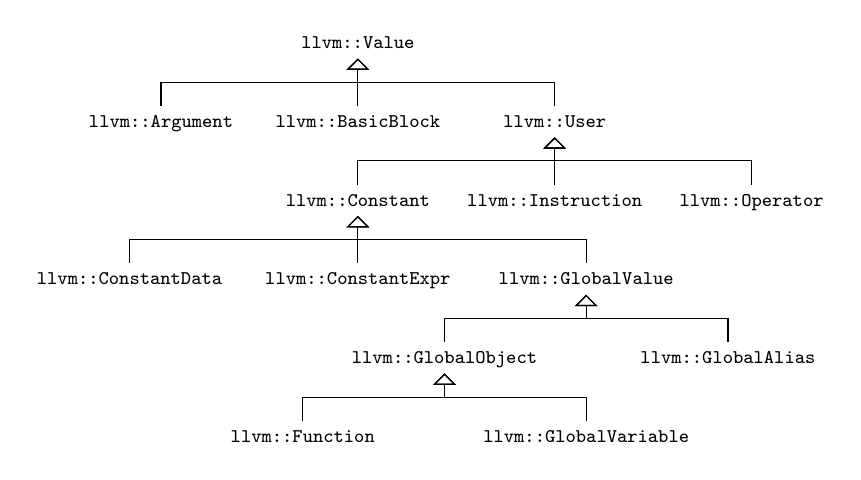
\begin{tikzpicture}
[
  every node/.style={
    font=\tt\scriptsize,
    text depth=0pt
  },
  extends/.style={
    draw,
    open triangle 90-
  },
  level distance=10mm,
  sibling distance=25mm,
  level 3/.style={
    sibling distance=29mm
  },
  level 4/.style={
    sibling distance=36mm
  },
]

\node{llvm::Value}
  [edge from parent fork down,
   edge from parent/.style={extends}]

  child{ node{\cppinline{llvm::Argument}} }
  child{ node{\cppinline{llvm::BasicBlock}} }
  child{ node{\cppinline{llvm::User}}
  	child{ node{\cppinline{llvm::Constant}}
			child{ node{\cppinline{llvm::ConstantData}} }
			child{ node{\cppinline{llvm::ConstantExpr}} }
			child{ node{\cppinline{llvm::GlobalValue}} 
				child{ node{\cppinline{llvm::GlobalObject}} 
					child{ node{\cppinline{llvm::Function}} }
					child{ node{\cppinline{llvm::GlobalVariable}} }
				}
				child{ node{\cppinline{llvm::GlobalAlias}} }
			}
		}
		child{ node{\cppinline{llvm::Instruction}} }
		child{ node{\cppinline{llvm::Operator}} }
  };
\end{tikzpicture}
\\
\pause
\bigskip
Something is missing...
\end{frame}


\begin{frame}{LLVM-IR}{Static Single Assignment}
LLVM-IR is SSA-based:

\begin{itemize}
\item every register is \alert{statically assigned} exactly \alert{once}
\end{itemize}
\bigskip
Statically means that:

\begin{itemize}
\item inside each function...
\item ...for each variable \llvminline{\%foo}...
\item ...there is \alert{only one} statement in the form \llvminline{\%foo = ...}
\end{itemize}
\bigskip
\alert{Static} (compile time) $\neq$ \alert{dynamic} (runtime)
{\footnotesize
\begin{itemize}
\item Single \emph{Dynamic} Assignment:\\\emph{in the execution trace} there is only one assignment to a variable \texttt{x}
\item Single \emph{Static} Assignment:\\\emph{in the code listing} there is only one assignment to a variable \texttt{x}
\begin{itemize}
\scriptsize
\item Assignments \alert{can} be performed multiple times (in a loop for example)
\end{itemize}
\end{itemize}
}
\end{frame}


\begin{frame}{Static Single Assignment}{Examples}
\begin{block}{Scalar SAXPY}
\cinput[\ttfamily\small]{snippet/scalar-saxpy.c}
\end{block}

\begin{block}{Scalar LLVM SAXPY}
\llvminput[\ttfamily\small]{snippet/scalar-saxpy.ll}
\end{block}

Temporary \llvminline{\%1} not reused! \llvminline{\%2} is used for the second
assignment!
\end{frame}


\begin{frame}{Static Single Assignment}{Examples}
\begin{block}{Array SAXPY}
\cinput[\ttfamily\scriptsize]{snippet/array-saxpy.c}
\end{block}

\begin{block}{Array LLVM SAXPY}
\llvminput[\ttfamily\scriptsize]{snippet/array-saxpy.ll}
\end{block}

One assignment for loop counter \llvminline{\%i.0}
\end{frame}

\begin{frame}{Static Single Assignment}{Handling Multiple Assignments}
\begin{block}{Max}
\cinput[\ttfamily\scriptsize]{snippet/max.c}
\end{block}

\begin{block}{LLVM Max -- WRONG}
\llvminput[\ttfamily\scriptsize]{snippet/bad-max.ll}
\end{block}

Why is it \alert{wrong}?
\end{frame}


\begin{frame}{Static Single Assignment}{Use \llvminline{phi} to Avoid Troubles}
The \llvminline{\%2} variable must be statically assigned once!\\
How do we handle conditional assignments then?

\begin{block}{LLVM Max}
\llvminput[\ttfamily\footnotesize]{snippet/good-max.ll}
\end{block}

The \llvminline{phi} instruction is a \emph{conditional move}:

\begin{itemize}
\item it takes $(\textrm{variable}_i, \textrm{label}_i)$ pairs
\item if coming from predecessor identified by $\textrm{label}_i$, its value is $\textrm{variable}_i$
\end{itemize}
\end{frame}


\begin{frame}{Static Single Assignment}{Definition and Uses}
Each SSA variable is assigned only once:

\begin{itemize}
\item variable \alert{definition}
\end{itemize}

\vfill
Each SSA variable can be referenced by multiple instructions:

\begin{itemize}
\item variable \alert{uses}
\end{itemize}

\vfill
Algorithms and technical language abuse of these terms!

\vfill
\emph{
Let \llvminline{\%foo} be a variable. If the definition of \llvminline{\%foo} does not
have side-effects nor uses, the aforementioned \llvminline{\%foo} variable 
can be erased from the CFG without altering program semantics.
}
\end{frame}


\begin{frame}{SSA \& LLVM-IR}{Static Single Assignment}
\large
\begin{block}{\centering Important observation}
\centering
SSA means that\\
\alert{there is always a 1:1 correspondence}\\
\alert{between a register and the instruction that assigns it}.
\end{block}
\bigskip
\begin{block}{\centering Consequence}
\centering
As a result, in LLVM-IR\\
\alert{registers are not separate objects}\\
but \alert{every LLVM Instruction\\is the output ``register'' of itself}.
\end{block}
\end{frame}


\begin{frame}{Static Single Assignment}{Rationale}
Old compilers are not SSA-based:

\begin{itemize}
\item converting non-SSA input into SSA form is expensive
\item cost must be amortized
\end{itemize}

\vfill
New compilers are SSA-based:

\begin{itemize}
\item SSA easier to work with
\item SSA-based analysis/optimizations are faster
\end{itemize}

%\vfill
%All modern compilers are SSA-based:
%
%\begin{itemize}
%\item exception are old version of the HotSpot Client compiler
%\end{itemize}
\end{frame}


% !TEX root = main.tex

\subsection{The Control Flow Graph}


\begin{frame}{A step back...}
Remember how we described the internal structure of an LLVM-IR module:
\begin{itemize}
\item \cppinline{llvm::Module} is a list of \cppinline{llvm::GlobalValue}s.
	\begin{itemize}
	\item \cppinline{llvm::Function} is a kind of \cppinline{llvm::GlobalValue}.
	\end{itemize}
\item \cppinline{llvm::Function} is a list of \cppinline{llvm::BasicBlock}s.
\item \cppinline{llvm::BasicBlock} is a list of \cppinline{llvm::Instruction}.
\end{itemize}
\bigskip
Functions and basic blocks act like containers:

\begin{itemize}
\item STL-like accessors: \cppinline{front()}, \cppinline{back()},
      \cppinline{size()}, \ldots
\item STL-like iterators: \cppinline{begin()}, \cppinline{end()}
\end{itemize}

\vfill
Each contained element is aware of its container:
\begin{itemize}
\item \cppinline{getParent()}
\end{itemize}
\vfill
Warning for BBs: order of iteration $\neq$ order of execution!
\end{frame}


\begin{frame}{A step back...}
In a \cppinline{llvm::BasicBlock}, the \cppinline{llvm::Instruction}s execute
in the order specified by the list.\\
\begin{itemize}
\item In which order do the \cppinline{llvm::BasicBlock}s execute?
\end{itemize}
\bigskip
The way the basic blocks are executed is implcitly described by
the \alert{branches} in each block.\\
\begin{itemize}
\item These branches describe the \alert{Control Flow Graph} of the function.
\end{itemize}
\end{frame}


\begin{frame}{Control Flow Graph}
LLVM automatically maintains a simple API for operating on the CFG:

\begin{itemize}
\item no need to run passes
\item no need to search the branch instructions in each basic block
\end{itemize}
\bigskip
Every CFG has an \alert{entry} basic block:

\begin{itemize}
\item the \alert{first} executed basic block
\item it is the \alert{root/source} of the graph
\item get it with \cppinline{llvm::Function::getEntryBlock()}
\end{itemize}

\end{frame}


\begin{frame}{Control Flow Graph}{Walking}
At the end of a basic blocks there's always a \alert{terminator} instruction:
\begin{itemize}
\item \llvminline{ret}, \llvminline{br}, \llvminline{switch}, \llvminline{unreachable}, \ldots
\end{itemize}

\bigskip
More than one \alert{exit} block can be present in a function:

\begin{itemize}
\item they are the \alert{leaves/sinks} of the graph
\item their terminator instructions are always \llvminline{ret}s
\begin{enumerate}
\item \cppinline{llvm::BasicBlock::getTerminator()}
\item check the opcode of the terminator
\end{enumerate}
\end{itemize}
\end{frame}


\begin{frame}{Side Note}{Casting Framework}
For performance reasons, a custom casting framework is used:

\begin{itemize}
\item you cannot use \cppinline{static\_cast} and \cppinline{dynamic\_cast} with
      types/classes provided by LLVM
\end{itemize}

\begin{block}{LLVM Casting Functions}
\centering
\medskip
\begin{tabular}{rl}

Static cast of \cppinline{Y*} to \cppinline{X}  &
\cppinline{X *llvm::cast<X>(Y *)}                \\

Dynamic cast of \cppinline{Y*} to \cppinline{X}  &
\cppinline{X *llvm::dyn\_cast<X>(Y *)}            \\

Is \cppinline{Y*} an instance of \cppinline{X}?  &
\cppinline{bool llvm::isa<X>(Y *)} \\

\end{tabular}
\smallskip
\end{block}

Example:

\begin{itemize}
\item is \cppinline{BB} a sink?\\
      \cppinline{llvm::isa<llvm::ReturnInst>(BB.getTerminator())}
\end{itemize}
\end{frame}


\begin{frame}{Control Flow Graph}{Basic Blocks}
Every basic block \cppinline{BB} has one or more\footnote{see include/llvm/IR/CFG.h}:

\begin{description}[predecessors]
\item[predecessors] from \cppinline{pred\_begin(BB)} to
      \cppinline{pred\_end(BB)}
\item[successors] from \cppinline{succ\_begin(BB)} to
      \cppinline{succ\_end(BB)}
\end{description}

\vfill
Other convenience methods available in \cppinline{llvm::BasicBlock}:

\begin{itemize}
\item useful getters
\begin{itemize}
\item \cppinline{BasicBlock *getUniquePredecessor()}
\item \ldots
\end{itemize}
\item moving a basic block
\begin{itemize}
\item      \cppinline{moveBefore(llvm::BasicBlock *)}
\item      \cppinline{moveAfter(llvm::BasicBlock *)}
\end{itemize}
\item split a basic block:
\begin{itemize}
\item      \cppinline{splitBasicBlock(llvm::BasicBlock::iterator)}
\end{itemize}
\item \ldots
\end{itemize}
\end{frame}


\begin{frame}{Control Flow Graph}{Instructions}
The \cppinline{llvm::Instruction} class defines common operations: \\
\medskip
\begin{itemize}
\item getting an operand
\begin{itemize}
\item \cppinline{getOperand(unsigned)}
\end{itemize}
\end{itemize}
\vfill
Subclasses provide specialized accessors: \\
\medskip
\begin{itemize}
\item the \llvminline{load} instruction takes as operand the pointer to the memory to be loaded:
\begin{itemize}
\item      \cppinline{llvm::LoadInst::getPointerOperand()}
\end{itemize}
\end{itemize}
\end{frame}


\begin{frame}{Instructions}{Creating New Instructions}
Instructions are created using:

\begin{itemize}
\item constructors
\begin{itemize}
\item \cppinline{llvm::LoadInst::LoadInst(...)}
\end{itemize}
\item factory methods
\begin{itemize}
\item \cppinline{llvm::GetElementPtrInst::Create(...)}
\end{itemize}
\item the helper class \cppinline{llvm::IRBuilder}
\begin{itemize}
\item \cppinline{llvm::IRBuilder<> builder(insPoint);}\\
\cppinline{builder.CreateAdd(...);}
\end{itemize}
\end{itemize}
\vfill
\alert{Interface is not homogeneous!}\\
Some instructions support all methods, others support only one.
\end{frame}


\begin{frame}{Instructions}{Inserting New Instructions}
\vfill
Instructions can be inserted:
\vfill
\begin{itemize}
\item automatically by \cppinline{IRBuilder}
\begin{itemize}
\item insertion point is given at \cppinline{IRBuilder} instantiation
\end{itemize}
\bigskip
\item manually by appending to a basic block
\item manually by inserting after/before another instruction
\end{itemize}
\vfill
\end{frame}


\begin{frame}{From Control Flow to Data Flow}{Definitions and Uses}
In LLVM, the data flow generated by the various instructions is represented by a simple hierarchy:

\begin{description}[valueMMM]
\item[value] something that can be used: \cppinline{llvm::Value}
\item[user] something that can use: \cppinline{llvm::User}
\item[use] the link between the \alert{value} and the \alert{user}: \cppinline{llvm::Use}
\end{description}
\medskip
A value is a \alert{definition}:

\begin{itemize}
\item Visiting where a definition is used:
\begin{itemize}
\item \cppinline{llvm::Value::use\_begin()}, \cppinline{llvm::Value::use\_end()}
\end{itemize}
\end{itemize}
\medskip
An user accesses \alert{definitions}:

\begin{itemize}
\item Visiting the definitions that are used:
\begin{itemize}
\item \cppinline{llvm::User::op\_begin()}, \cppinline{llvm::User::op\_end()}
\end{itemize}
\end{itemize}
\medskip

\end{frame}


\begin{frame}{From Control Flow to Data Flow}{Instructions are Values}
\vfill
\begin{itemize}
\item \cppinline{llvm::Value} inherits from \cppinline{llvm::User}
\item \cppinline{llvm::Instruction} inherits from \cppinline{llvm::Value}
\begin{itemize}
\normalsize
\item[$\Rightarrow$] The value produced by the instruction is\\the \alert{instruction itself}!
\end{itemize}
\end{itemize}

\begin{block}{Example}
\begin{center}
\llvminline{\%6 = load i32, i32* \%1, align 4}\\
\medskip
The \llvminline{load} is described by an instance of \cppinline{llvm::Instruction}. \\
That instance also represents the \llvminline{\%6} variable. \\
\end{center}
\end{block}

\begin{center}
Not all instances of \cppinline{llvm::Value} are also \cppinline{llvm::Instruction}s!\\
\smallskip
{\small i.e. function arguments}

\end{center}
\vfill
\end{frame}


\begin{frame}{From Control Flow to Data Flow}{Value Typing}
Every \cppinline{llvm::Value} is typed:

\begin{itemize}
\item use \cppinline{llvm::Value::getType()} to get the type
\end{itemize}

\vfill
Since every instruction is a value:

\begin{itemize}
\item instructions are typed
\end{itemize}

\vfill
\begin{block}{Example}
\begin{center}
\llvminline{\%6 = load i32, i32* \%1, align 4}\\
\medskip
The type of the \llvminline{\%6} variable is the type of the return value of the \llvminline{load} instruction, \llvminline{i32}\\
\end{center}
\end{block}
\end{frame}


%\begin{frame}{From Control Flow to Data Flow}{Instructions are like functions}
%\vfill
%\vfill
%\begin{columns}[t]
%\column{.45\textwidth}
%Functions:
%
%\begin{itemize}
%\item used by call sites
%\item uses formal parameters
%\end{itemize}
%
%\column{.45\textwidth}
%Instructions:
%
%\begin{itemize}
%\item define an SSA value
%\item uses operands
%\end{itemize}
%\end{columns}
%
%\vfill
%\vfill
%\end{frame}




% !TEX root = 01.tex

\section{Conclusions}
\begin{frame}{Conclusions}
LLVM is a \alert{production-quality} compiler framework:

\begin{itemize}
\item[$\Rightarrow$] impossible knowing all details
\end{itemize}

\vfill
But:

\begin{itemize}
\item it is well organized
\item given you known compilers theory, it is relatively easy to find what you need inside its sources
\end{itemize}

\vfill
Please take into account C++:
\begin{itemize}
\item basic skills required
\end{itemize}
\end{frame}



\section{Bibliography}
\begin{frame}[allowframebreaks]{Bibliography}
\nocite{*}
\bibliographystyle{unsrt}
\bibliography{bibliography}
\end{frame}


\end{document}
